\FloatBarrier
\subsection{Question 1}
Our reference model is based on the approach presented in the textbook and is implemented as $sys_{ref}=tf(beta*B,Am,Gz.Ts)$, where $beta*B$ is chosen such that the step response of the reference model approaches 1. We define $A_o =  [0 ,0]$ and compute $ Ac = poly([A0 ,roots(Am)'])$.

\autoref{code:str11} outlines the necessary steps to compute the control output. The system polynomials are estimated using the Recursive Least Squares (RLS) method, and the $R$ and $S$ polynomials are determined using the Diophantine equation. \autoref{fig:str11} shows the system output and control effort for the indirect STR without zero cancellation, while \autoref{fig:str12} illustrates the evolution of parameter estimates over the course of the simulation.


\begin{code}
	\begin{matlabcode}{firstnumber = 1}
%% Parameters
cancel = 0; % 0 no zero cancel, 1 all zero cancel
noise = 0; % if 1 white noise, 2 colored noise
distrubance = 1; % set to 1 for step disturbance
distrubance_fix = 0; % set to 1 to fix system
integral_fix = 0; % set 1 to limit u
vlimit = 4; % limit of u
lamda = 1;

beta = sum(Am)/sum(B);
sys_ref_dis = tf(beta*B,Am,Gz.Ts) ;
. . .
for i = Nv+1:N
	
	y(i) =-A(2:end)*y(i-1:-1:i-na)+B*(u(i-d0:-1:i-na)+vdist(i-(numel(A)-numel(B)):-1:i-(numel(A)-1))+ynoise(i-(numel(A)-numel(B)):-1:i-(numel(A)-1))) ;
	Y = [-y(i-1) , -y(i-2), -y(i-3)];
	U = [u(i-1)+vdist(i-1), u(i-2)+vdist(i-2), u(i-3)+vdist(i-3)] ;
	
	[teta , P] = RLS(Y ,U , y(i) , teta , P , Nv,lamda) ;
	tetas(:,i)=teta;
	
	Aes = [1 teta(1:Nv/2)'] ;
	Bes = teta(Nv/2+1:end)' ;
	
	[R , S] = Diophantine(Aes , Bes , Ac)  ;
	AcBm = conv(Ac , Bm) ;
	AmB = conv(Am , Bes) ;
	T = [(sum(AcBm) / sum(AmB))*poly(A0)] ;
	
	u(i) = (-R(2:end)*u(i-1:-1:i-(numel(R)-1))+T*uc(i-(numel(R)-numel(T)):-1:i-(numel(R)-1))-S*y(i-(numel(R)-numel(S)):-1:i-(numel(R)-1)))/R(1) ;
end
	\end{matlabcode}
	\captionof{listing}{Basic impelementation of Indirect STR without zero cancellation}
	\label{code:str11}
\end{code}

\begin{figure}
	\centering
	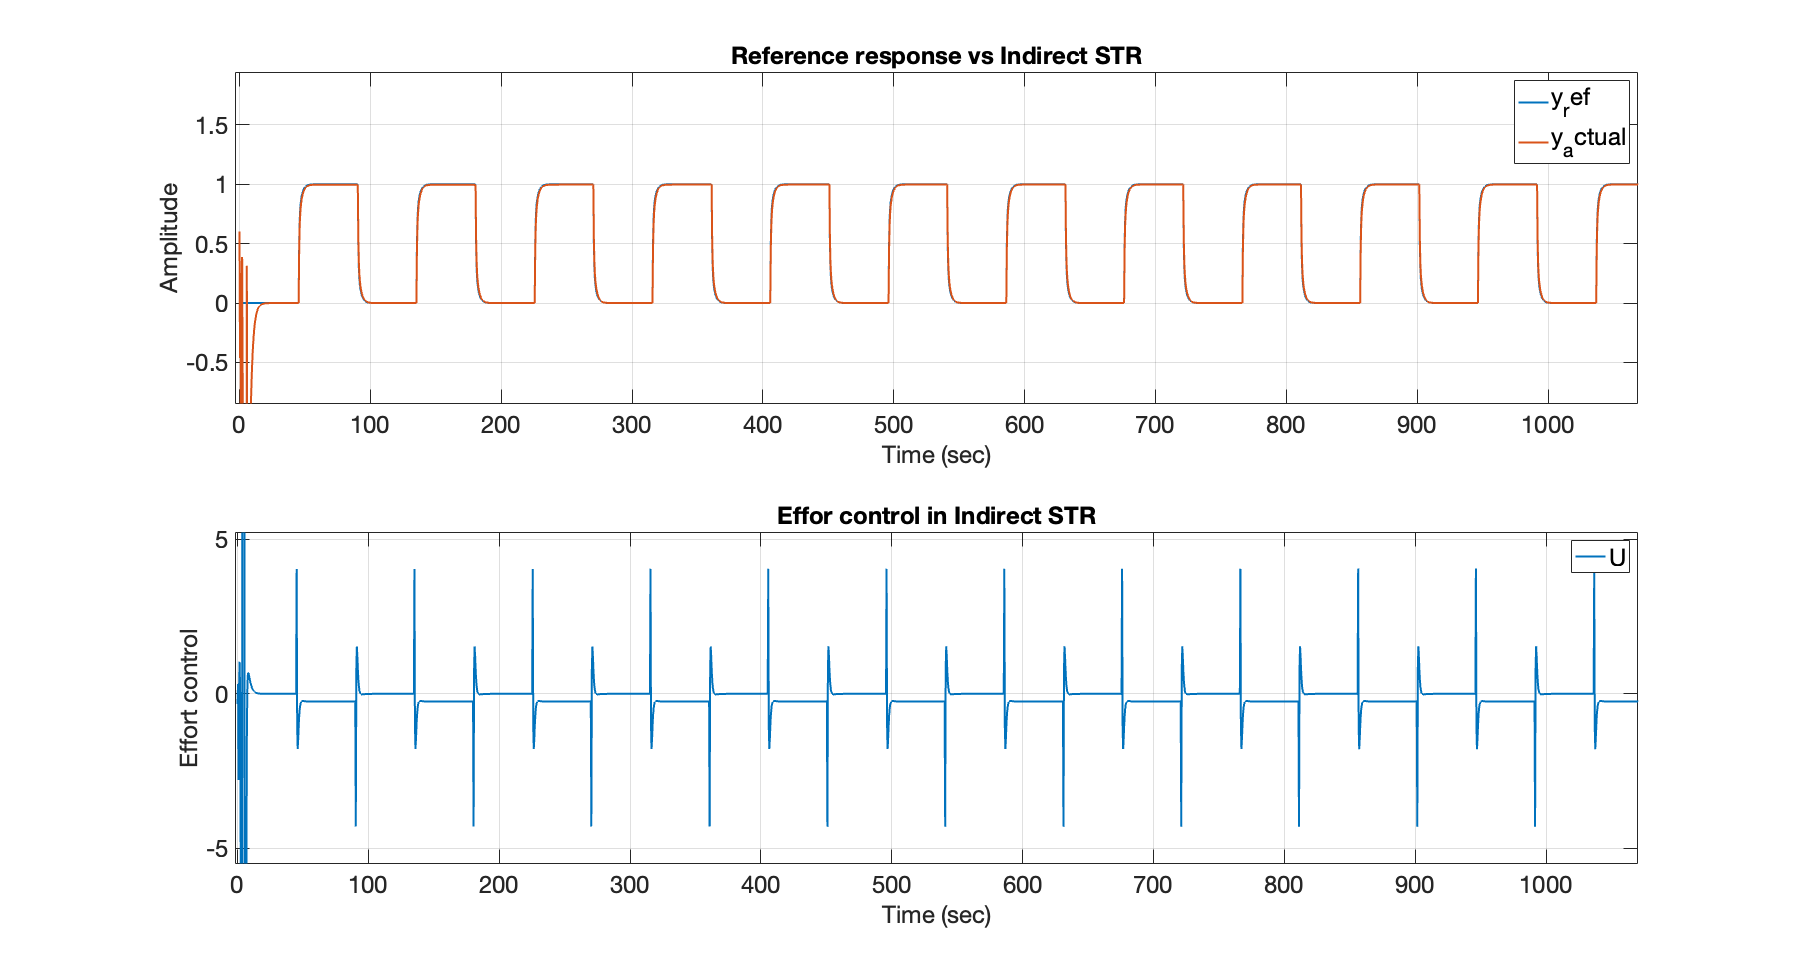
\includegraphics[width=\textwidth]{images/str11.png}
	\caption{System response without zero cancelling Indirect STR }
	\label{fig:str11}
\end{figure}

\begin{figure}
	\centering
	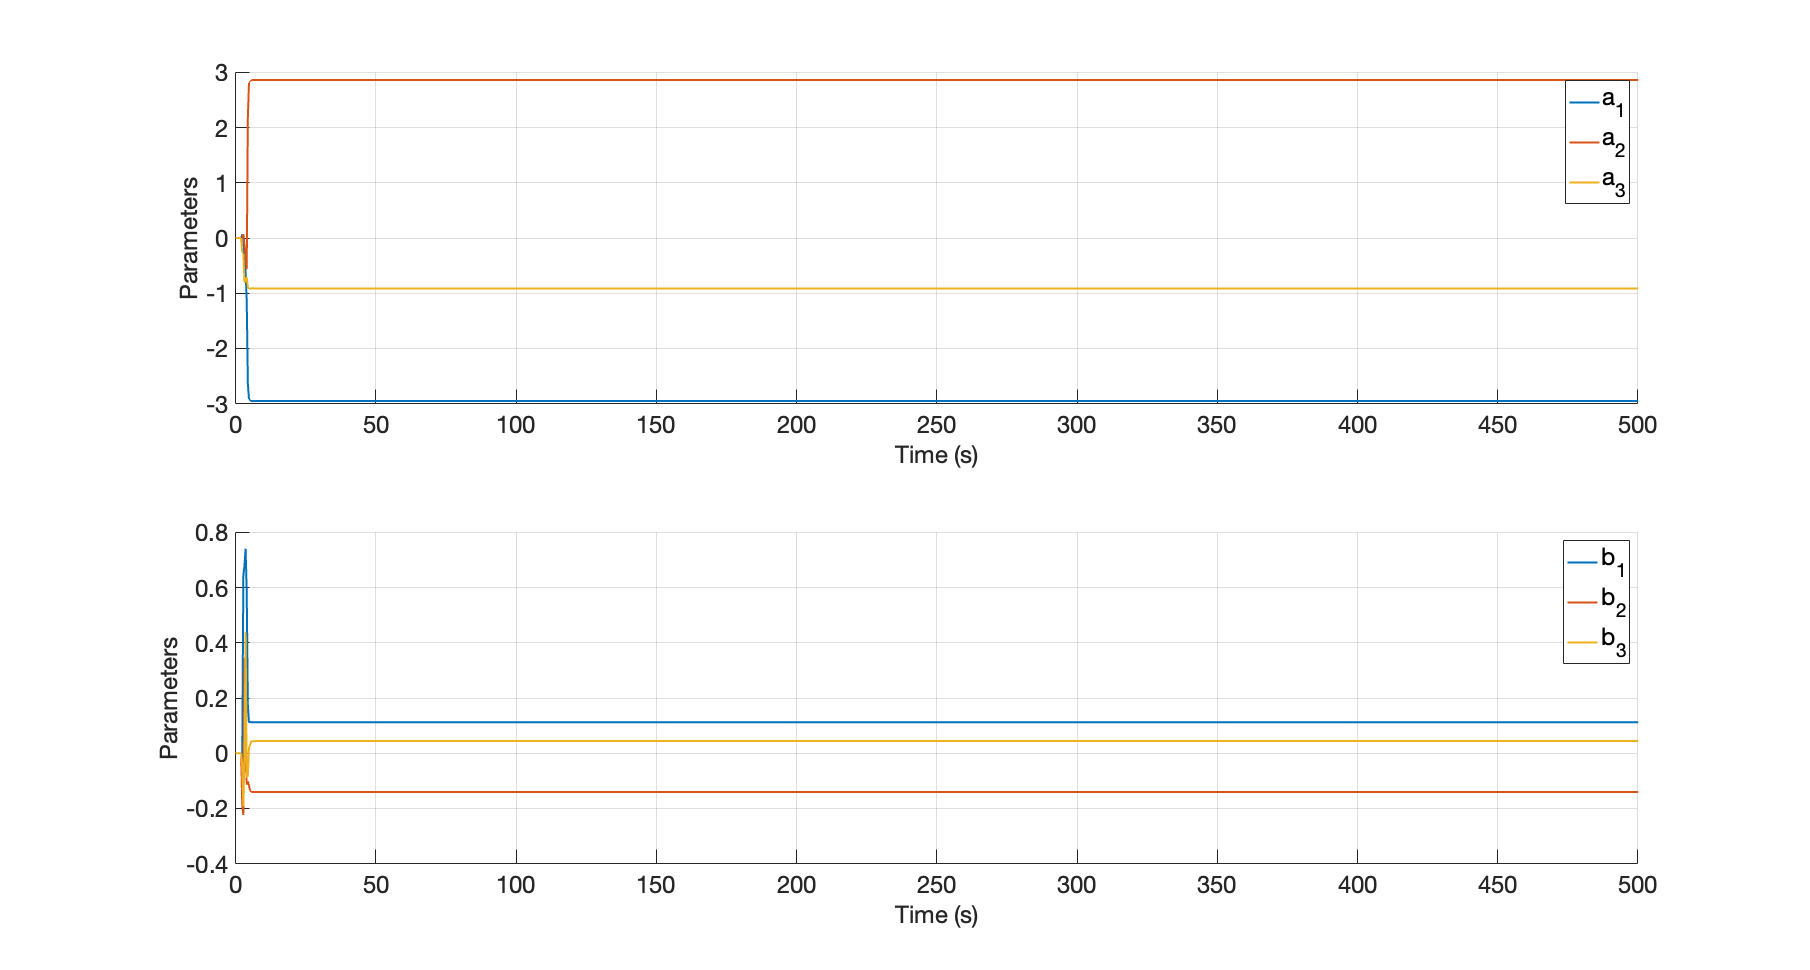
\includegraphics[width=\textwidth]{images/str12.png}
	\caption{System parameters in indirect STR without zero cancellation}
	\label{fig:str12}
\end{figure}

The code for this section is available at \lstinline|assignment2/part2/STR1_indirect.m|.  The Diophantine equation solver code is at \lstinline|assignment2/part2/Diophantine.m| and RLS impelementation is located at \lstinline|assignment2/part2/RLS.m|.
